\section{E-commerce Concepts}
\label{sec:ecommerce}

In the layer of e-commerce concepts,
each node represents a specific shopping scenario,
which can be interpreted by at least one primitive concept.
In this section,
we first introduce the high criteria of a good e-commerce concept using several examples, 
then show how we generate all those e-commerce concepts  and further propose an algorithm to link e-commerce concepts to the layer of primitive concepts.



\subsection{Criteria}

As introduced in \secref{sec:overview},
user needs are conceptualized as e-commerce concepts in AliCoCo, and a good e-commerce concept should satisfy the following criteria:

\noindent
\textbf{(1) E-commerce Meaning.}
It should let anyone easily think of some items in the e-commerce platform, which means it should naturally represent a particular shopping need. Phrases like ``blue sky'' or ``hens lay eggs'' are not e-commerce concepts, 
because we can hardly think of any related items.

\noindent
\textbf{(2) Coherence.}
It should be a coherent phrase. Counter-examples can be 
``gift grandpa for Christmas'' or ``for kids keep warm'',
while the coherent ones should be ``Christmas gifts for grandpa'' and ``keep warm for kids''.

\noindent
\textbf{(3) Plausibility.}
It should be a plausible phrase  according to commonsense knowledge. Counter-examples can be ``sexy baby dress'' or 
``European Korean curtain'' since we humans will not describe a dress for babies using the word ``sexy'' and a curtain can not be in both European style and Korean style.

\noindent
\textbf{(4) Clarity.}
The meaning of an e-commerce concept should be clear and easy to understand.
Counter-examples can be ``supplementary food for children and infants'' where the subject of this can be either older-aged children or newborns. This may lead to a confusion for our customers.

\noindent
\textbf{(5) Correctness.}
It should have zero pronunciation or grammar error.

\subsection{Generation}

There is no previous work on defining such e-commerce concepts and few on mining such phrases from texts. 
In practice, we propose a two-stage framework: 
firstly we use two different ways to generate large amount of possible e-commerce concept candidates,
then a binary classification model is proposed to 
identify those concepts which satisfy our criteria.

\subsubsection{Candidate Generation}
There are two different ways to generate concept candidates. 
The first is mining raw concepts from texts.
In practice, we adopt AutoPhrase\cite{shang2018automated} to mine possible concept phrases from large corpora in e-commerce including search queries, product titles, user-written reviews and shopping guidance written by merchants.
Another alternative is to generating new candidates using existing primitive concepts\footnote{If a primitive concept satisfies all five criteria, it can be regarded as an e-commerce concept as well.}. 
For example, we combine ``\textit{Location: Indoor}'' with ``\textit{Event: Barbecue}'' to get a new concept ``indoor barbecue'', which is not easy to be mined from texts since it's a little bit unusual.
However, it is actually a quite good e-commerce concept 
since one goal of AliCoCo is to cover as many user needs as possible.
The rule to combine different classes of primitive concepts is using some automatically mined then manually crafted patterns.
For example, we can generate a possible concept ``warm hat for traveling'' using a pattern ``[\textit{class: Function}] [\textit{class: Category}] for [\textit{class: Event}]''.
\tabref{tab:pattern} shows some patterns used in practice and corresponding e-commerce concepts, including some bad ones waiting to be filtered out in the following step.

\begin{table*}[th]
	\centering
	\small
	\begin{tabular}{|l|c|c|}
		\hline
		\bi{Pattern} & \bi{Good Concept} & \bi{Bad Concept} \\
		\hline
		[\textit{class: Function}] [\textit{class: Category}] for [\textit{class: Event}] & warm hat for traveling & warm shoes for swimming \\
		\hline
		[\textit{class: Style}] [\textit{class: Time->Season}] [\textit{class: Category}] & British-style winter trench coat &
		casual summer coat \\
		\hline
		[\textit{class: Location}] [\textit{class: Event->Action}] [\textit{class: Category}] & British imported snacks &
		Bird's nest imported from Ghan \\
		\hline
		[\textit{class: Function}] for [\textit{class: Audience->Human}] & health care for olds &
		waterproofing for middle school students \\
		\hline
		[\textit{class: Event->Action}] in [\textit{class: Location}]  &  traveling in European &
		Bathing in the classroom \\
		\hline
	\end{tabular}
	\caption{Some patterns used to generate e-commerce concepts.}
	\label{tab:pattern}
\end{table*}



\subsubsection{Classification}
\label{sec:classification}
To automatically judge whether a candidate concept satisfies the criteria of being a qualified e-commerce concept or not, 
the main challenge is to test its plausibility.
For the other four criteria,
character-level and word-level language models
and some heuristic rules are able to meet the goal.
However, it is difficult for machines to grasp
commonsense knowledge as we humans do to 
know that ``sexy'' is not suitable to describe a dress when it's made for a child.
Moreover, the lack of surrounding contexts makes the problem more challenging, since our concepts are too short (2-3 words on average).

To tackle this problem, 
we propose a knowledge-enhanced deep classification model to first link each word of a concept to an external knowledge base then introduce rich semantic information from it.
The model architecture is shown in \figref{fig:classification},
which is based on Wide\&Deep \cite{cheng2016wide} framework.
The input is a candidate concept $c$, 
and the output is a score, measuring the probability of $c$ being a good e-commerce concept.
In this paper, we denote a char as a single Chinese or English character,
and a segmented word (or term) is a sequence of several chars such as ``Nike'' or ``牛仔裤 (jeans)''.
We perform Chinese word segmentation for all the input concepts before feeding to the model.

\begin{figure}[th]
	\centering
	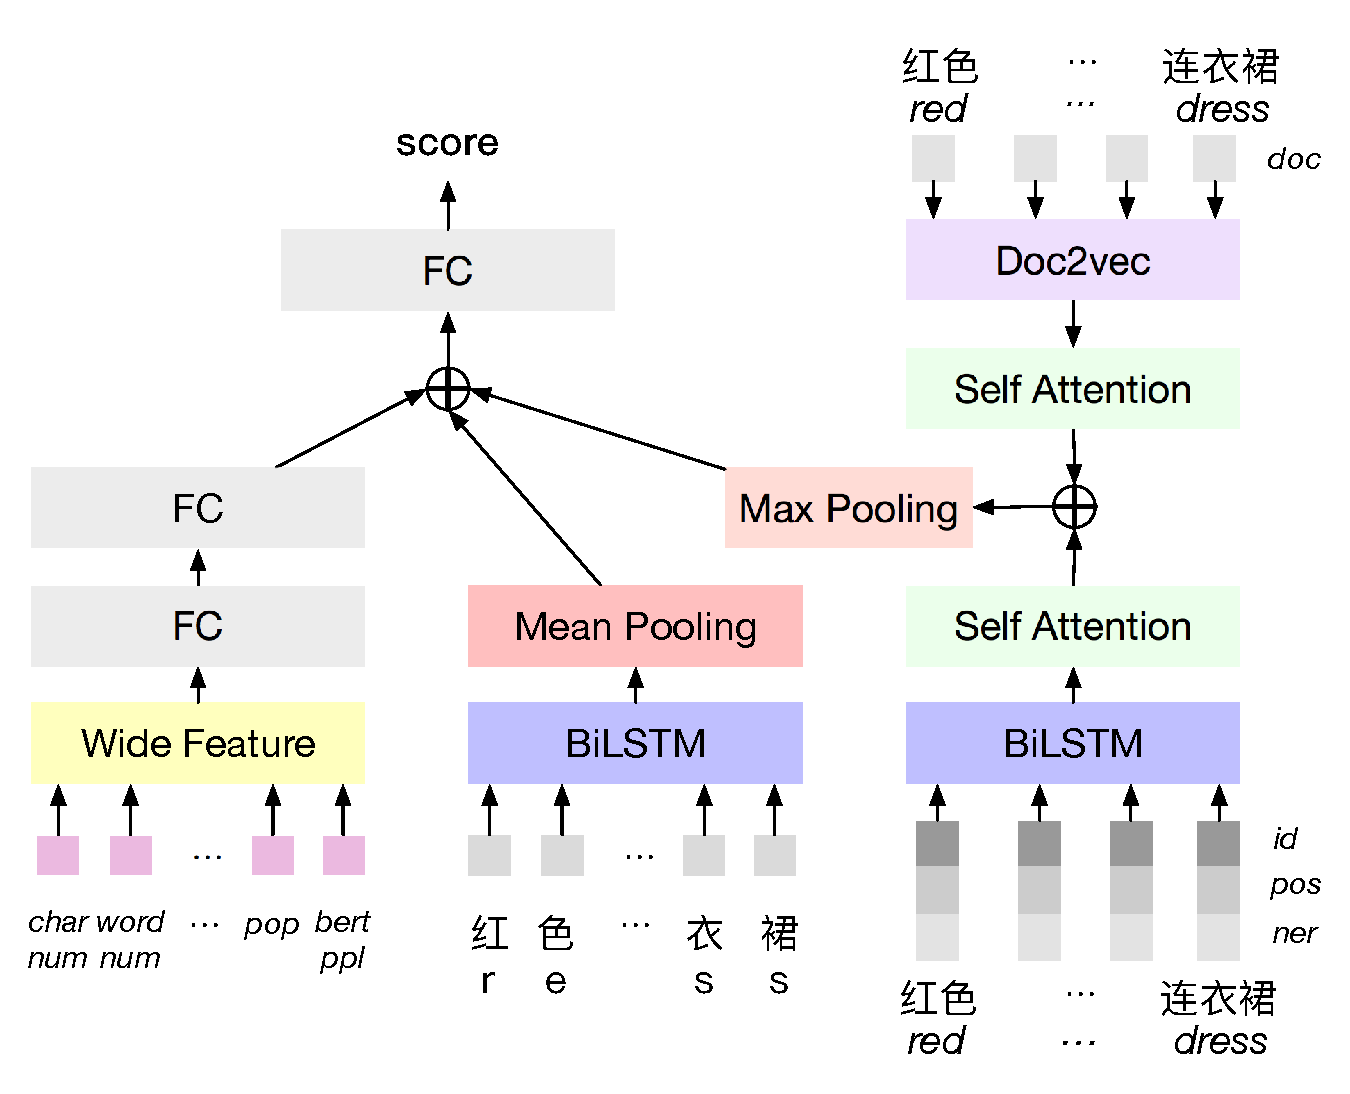
\epsfig{file=figures/classification.eps, width=\columnwidth}
	\caption{Overview of knowledge-enhanced deep model for e-commerce concept classification.
	}
	\label{fig:classification}
\end{figure}


In the Deep side,
there are mainly two components.
Firstly, a char level BiLSTM is used to encode the candidate concept $c$
by feeding the char-level embedding sequence $\{\bi{ch}_1, \bi{ch}_2,...\bi{ch}_n\}$
after simple embedding lookup.
After mean pooling,
we get the concept embedding $\bi{c}_1$.
The other component is knowledge-enhanced module.
The input consists of there parts:
1) pre-trained word embeddings; 2) POS tag \cite{toutanova2003feature} embedding using a lookup table; 3) NER label \cite{finkel2005incorporating} embedding using a lookup table.
After concatenate those three embeddings, 
we obtain the input embedding sequence of candidate concept $c$: 
$\{\bi{w}_1, \bi{w}_2,...\bi{w}_m\}$ ($m<n$).
After going through BiLSTM, we use self attention mechanism \cite{vaswani2017attention} to further encode the mutual influence of each word within the concept and get a sequence output 
$\{\bi{w'}_1, \bi{w'}_2,...\bi{w'}_m\}$.
To introduce external knowledge into the model to do commonsense reasoning on short concepts,
we link each word $w$ to its corresponding Wikipedia article if possible.
For example, ``性感 (sexy)'' can be linked to \url{https://zh.wikipedia.org/wiki/%E6%80%A7%E6%84%9F}
	(\url{https://en.wikipedia.org/wiki/Sexy}).
Then we extract the gloss of each linked Wikipedia articl as the external knowledge to enhance the feature representation of concept words.
A gloss is a short document to briefly introduce a word.
We employ Doc2vec \cite{le2014distributed} to encode each extracted gloss for word $\bi{w}_i$ as $\bi{k}_i$.
Then, we get the representation of the knwoledge sequence after a self attention layer:
$\{\bi{k'}_1, \bi{k'}_2,...\bi{k'}_m\}$.
We concatenate  $\bi{w'}_i$ as $\bi{k'}_i$ and use max-pooling to get the final knowledge-enhanced representation of candidate concept $\bi{c}_2$.

In the Wide side, 
we mainly adopt pre-calculated features such as the number of characters and words of candidate concept,
the perplexity of candidate concept calculated by 
a BERT \cite{devlin2018bert} model specially trained on e-commerce corpus, and other features like the popularity of each word appearing in e-commerce scenario.
After going through two fully connected layers, 
we get the wide feature representation $\bi{c}_3$.

The final score $\hat y_c$ is calucalated by concatenating the three embedding $\bi{c}_1$, $\bi{c}_2$ and $\bi{c}_3$ then going through a MLP layer.
We use point-wise learning with the negative log-likelihood objective function to learn the parameters of our model:
\begin{equation}
\mathscr{L} = -\sum_{(c)\in D^+}{\log \hat y_c} + \sum_{(c)\in D^-}{\log (1-\hat y_c)}
\end{equation}
where $D^+$ and $D^-$ are the good and bad e-commerce concepts.

We expect this model can help filter out most of bad candidate concepts generated in the first step.
To strictly control the quality, we randomly sample a small portion of every output batch which passes the model checking to ask domain experts to manually annotate.
Only if the accuracy riches a certain threshold,
the whole batch of concepts will be added into AliCoCo.
Besides, the annotated samples will be added to training data to iteratively improve the model performance.



%Mining useful concept phrases is the fundamental task to construct our concept net. 
%Texts in e-commerce include search queries, item titles, and item comments, which are very different from normal texts since they are short and extremely noisy, which increases the difficulty of mining valuable information.
%Besides, the algorithm has to achieve an acceptable precision since Crowdsourcing resource is limited.
%Another problem is that our ideal target is to cover all user needs, while the fact is: user needs seems endless. Thus, mining concept phrases is a continuous procedure.



\subsection{Understanding}
\label{sec:tagging}
For those good e-commerce concepts which are directly mined from text corpora,
they are isolated phrases waiting to be integrated into AliCoCo.
To better understand (or interpret) those user needs (aka. e-commerce concepts),
it is a vital step to link them to the layer of primitive concepts.
We call the main task as \textit{``e-commerce concept tagging''}.
Revisit the example shown in \secref{sec:overview}, 
given an surface from ``outdoor barbecue'', 
we need to infer that ``outdoor'' is a ``\textit{Location}'' and ``barbecue'' is an ``\textit{Event}''.
However, word ``barbecue'' can also be a movie in the layer of primitive concepts, so it may be recognized into the class of ``\textit{IP}''.
We formulate this task as a \textit{short text} Named Entity Recognition (NER) problem, which is more challenging to a normal NER task since
concept phrases here are too short (2-3 words on average).
Lack of contextual information make it harder to disambiguate between different classes.

To overcome the above challenges,
we propose a text-augmented deep NER model with fuzzy CRF,
shown in \figref{fig:tagging}.
The input of this task is a sequence of concept word $\{\bi{w}_1, \bi{w}_2,...\bi{w}_m\}$ after Chinese word segmentation, 
while the output is a sequence of same length $\{\bi{y}_1, \bi{y}_2,...\bi{y}_m\}$ denoting the class labels for each word with In/Out/Begin (\textbf{I/O/B}) scheme.
The model consisting of two components: text-augmented concept encoder and fuzzy CRF layer.

\begin{figure}[th]
	\centering
	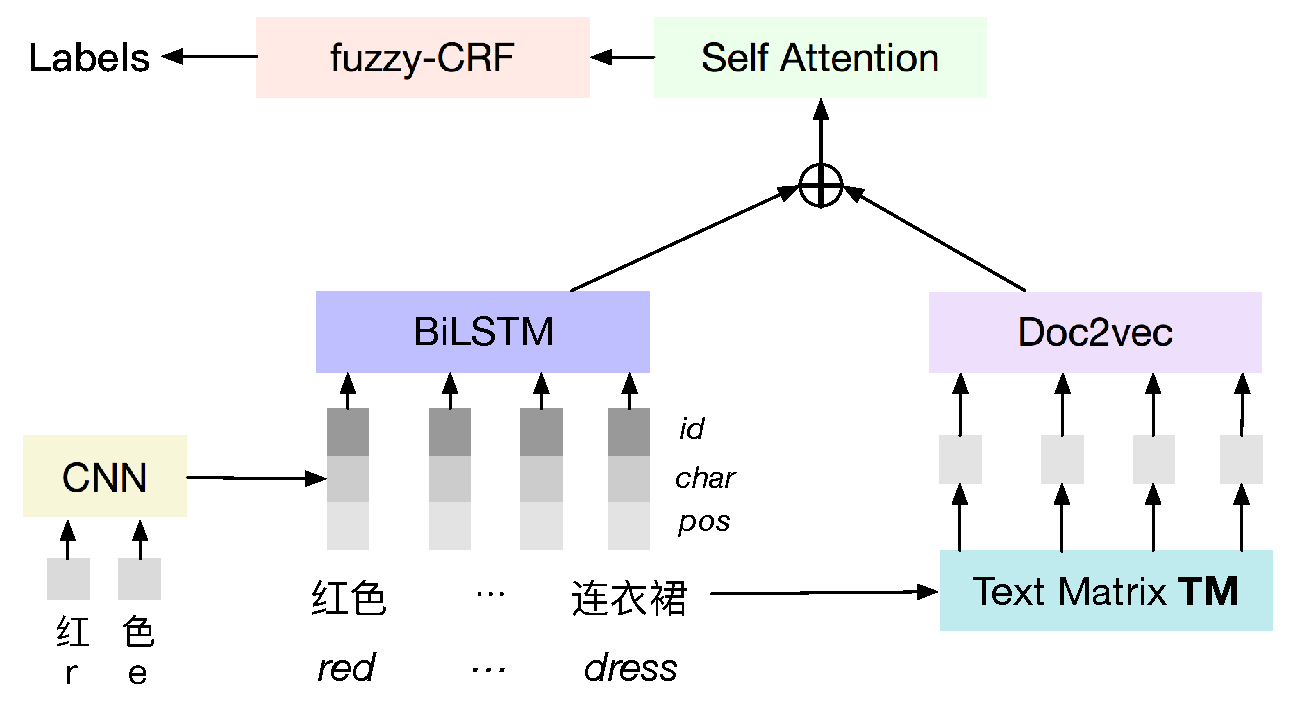
\epsfig{file=figures/tagging.eps, width=\columnwidth}
	\caption{Overview of text-augmented deep NER model for e-commerce concept tagging.
	}
	\label{fig:tagging}
\end{figure}


\subsubsection{Text-augmented concept encoder}
To leverage informative features in the representation layer,
we employ word-level, char-level features and position features.
We randomly initialize a lookup table to obtain an embedding for every character. Let $C$ be the vocabulary of characters, a word $w_i$ can be represented as a sequence of character vectors: $\{\bi{c}_1^i, \bi{c}_2^i, ..., \bi{c}_t^i\}$, where $\bi{c}_j^i$ is the vector for the $j$-th character in the word $w_i$ and $t$ is the word length. 
Here we adopt a convolutional neural network (CNN)  architecture to extract the char-level features $\bi{c}_i$ for each word $w_i$. 
Specifically, we use a convolutional layer with window size $k$ to involve the information of neighboring characters for each character.
A max pooling operation is then applied to output the final character representation as follows:
\begin{equation}
	 \bi{c}^i_j = \cnn([\bi{c}_{j-k/2}^i, ..., \bi{c}_j^i, ..., \bi{c}_{j+k/2}^i])
\end{equation}
\begin{equation}
	\bi{c}_i = \maxpool([\bi{c}^i_0, ... \bi{c}^i_j, ...]) 
\end{equation}
To capture word-level features, we use pre-trained word embeddings from GloVe \cite{pennington2014glove} to map a word into a real-valued vector $\bi{x}_i$ , as the initialized word features and will be fine-tuned during training. 
Furthermore,
we calculate part-of-speech tagging features $\bi{p}_i$.
Finally, we obtain the word representation $\bi{w}_i$ by concatenating three embeddings:
\begin{equation}
\bi{w}_i =[\bi{x}_i;\bi{c}_i;\bi{p}_i].
\end{equation}
Similar to the classification model introduced in the previous task,
we feed the sequence of word representations to BiLSTM layer to obtain hidden embeddings $\{\bi{h}_1, \bi{h}_2, ..., \bi{h}_m\}$.
To augment our model with more textual information,
we construct a textual embedding matrix $\textbf{TM}$ by mapping each word back to large-scale text corpus to extract surrounding contexts and encode them via Doc2vec.
Thus, we lookup each word $w_i$ in $\textbf{TM}$ to obtain a text-augmented embedding $\bi{tm}_i$.
We concatenate $\bi{h}_i$ and $\bi{tm}_i$ then use a self attention layer to adjust the representations of each words by considering the augmented textual embeddings of surrounding words, aiming to obtain better feature representations for this task:
\begin{equation}
\bi{h'}_i =\selfatt([\bi{h}_i;\bi{tm}_i]).
\end{equation}


\subsubsection{Fuzzy CRF layer}

\begin{figure}[th]
	\centering
	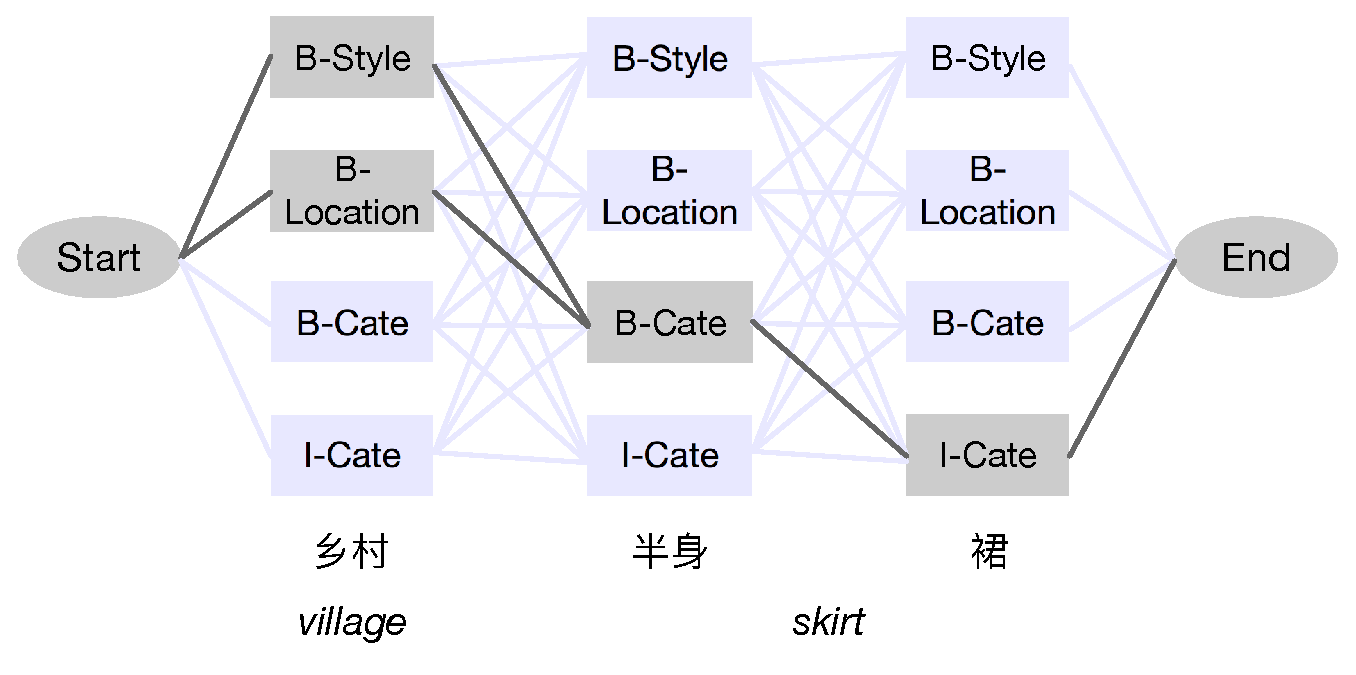
\epsfig{file=figures/fuzzy.eps, width=\columnwidth}
	\caption{A real example in fuzzy CRF layer.}
	\label{fig:fuzzy}
\end{figure}

Following the concept encoding module, 
we feed the embeddings to a CRF layer.
Different from normal CRF,
%(\eqnref{eqn:crf1}, \eqnref{eqn:crf2}, \eqnref{eqn:crf3}),
we use a fuzzy CRF \cite{shang2018learning} to better handle the disambiguation problem since the valid class label of each word is not unique and this phenomenon is more severe in this task since our concept is too short.
\figref{fig:fuzzy} shows an example, where 
the word ``乡村 (village)'' in the e-commerce concept ``乡村半身裙 (village skirt)'' can linked to the primitive concept ``\textit{空间: 乡村 (Location: Village)}'' or ``\textit{风格: 乡村 (Style: Village)}''.
They both make sense.
Therefore, we adjust the final probability 
as 
\begin{equation}
L(y|\bi{X}) = \frac{\sum_{\hat y \in Y_{possible}}e^{s(X, \hat y)}} {\sum_{\hat y \in Y_{X}}e^{s(X, \hat y)}}.
\end{equation}
where $Y_{X}$ means all the possible label sequences for sequence $X$, and $Y_{possible}$ contains all the possible label sequences.






